Zunächst wird für dieses Verfahren die Analyse mit der Durchlichtauswertung durchgeführt.
Aus dem Grund werden nur transparente Brillengläser untersucht.
In Abbildung \ref{tikz:abbStreifenaufnahmen} werden einzelne Aufnahmen der Brillengläser, bei Verwendung des Aufbaus aus dem linken Teilbild aus Abbildung \ref{tikz:abbAufbauFotos}, dargestellt.
Dabei wurden die Brillengläser auf eine dunkle Halterung gelegt, welche im linken Teilbild aus Abbildung \ref{tikz:abbAufbauFotos} über dem Bildschirm zu erkennen ist.

% Abbildung: Streifenaufnahmen
{
	\begin{figure}[H]
		\centering
		\begin{adjustbox}{width=\textwidth}
	\begin{tikzpicture}[every node/.style={inner sep=0,outer sep=0}]
		% Bilder
		\node [anchor=north west] (img1) at (0,0) {\includegraphics[frame,width=.31\textwidth]{05_ergebnisse/ergSichtpruefungDurchLichtstreuung/durchlichtAuswertungLichtstreuung/figures/gefärbtesBrillenglas2_rotiert_Bild}};
		\node [anchor=north west] (img2) at (0.345\textwidth,0) {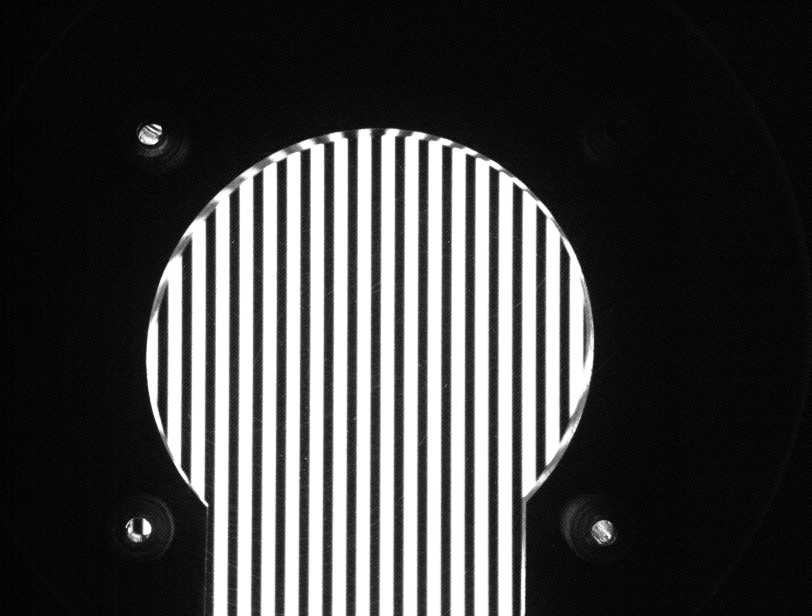
\includegraphics[frame,width=.31\textwidth]{05_ergebnisse/ergSichtpruefungDurchLichtstreuung/durchlichtAuswertungLichtstreuung/figures/polierfehler}};
		\node [anchor=north west] (img3) at (0.69\textwidth,0) {\includegraphics[frame,width=.31\textwidth]{05_ergebnisse/ergSichtpruefungDurchLichtstreuung/durchlichtAuswertungLichtstreuung/figures/HS_Beschädigung}};
		
		% Captions
		\node [below=0.2cm of img1] (cap1) {Brillenglas 1};
		\node [below=0.2cm of img2] (cap2) {Brillenglas 2};
		\node [below=0.2cm of img3] (cap3) {Brillenglas 3};			
	\end{tikzpicture}
\end{adjustbox}
\caption[Aufnahmen der Streifenmuster beim Durchlichtverfahren]{Aufnahmen der Streifenmuster beim Durchlichtverfahren}
		\label{tikz:abbStreifenaufnahmen}
	\end{figure}
}

\noindent
Durch Anwendung des Verfahrens \glqq Sichtprüfung durch Lichtstreuung\grqq ~erhält man für die drei Brillengläser folgende Bilder:

% Abbildung: Ergebnis der Sichtprüfung durch Lichtstreuung
{
	\begin{figure}[H]
		\centering
		\begin{adjustbox}{width=\textwidth}
	\begin{tikzpicture}[every node/.style={inner sep=0,outer sep=0}]
		% Bilder
		\node [anchor=north west] (img1) at (0,0) {\includegraphics[frame,width=.31\textwidth]{05_ergebnisse/ergSichtpruefungDurchLichtstreuung/durchlichtAuswertungLichtstreuung/figures/gefärbtesBrillenglas2_rotiert_sichtpruefungLichtstreuung}};
		\node [anchor=north west] (img2) at (0.345\textwidth,0) {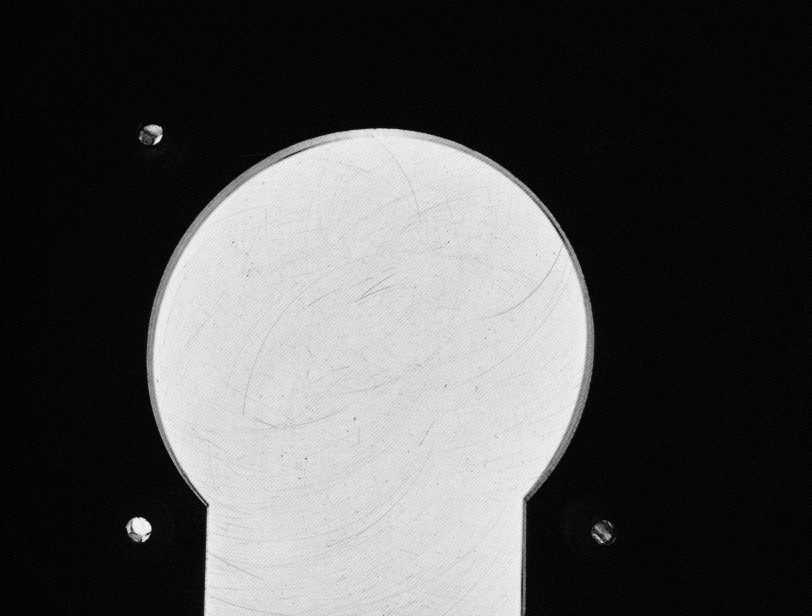
\includegraphics[frame,width=.31\textwidth]{05_ergebnisse/ergSichtpruefungDurchLichtstreuung/durchlichtAuswertungLichtstreuung/figures/polierfehler_ergebnis}};
		\node [anchor=north west] (img3) at (0.69\textwidth,0) {\includegraphics[frame,width=.31\textwidth]{05_ergebnisse/ergSichtpruefungDurchLichtstreuung/durchlichtAuswertungLichtstreuung/figures/HS_Beschädigung_ergebnis}};
		
		% Captions
		\node [below=0.2cm of img1] (cap1) {Brillenglas 1};
		\node [below=0.2cm of img2] (cap2) {Brillenglas 2};
		\node [below=0.2cm of img3] (cap3) {Brillenglas 3};			
	\end{tikzpicture}
\end{adjustbox}
\caption[Ergebnisbilder des Verfahrens \glqq Sichtprüfung durch Lichtstreuung\grqq]{Ergebnisbilder des Verfahrens \glqq Sichtprüfung durch Lichtstreuung\grqq}
		\label{tikz:abbCombinePatternPictures}
	\end{figure}
}

\noindent
Um die Bilder aus Abbildung \ref{tikz:abbCombinePatternPictures} zu erzeugen wurde als Verknüpfungsmethode des  Verfahrens die betragsmäßige Differenz gewählt, um einen hohen Kontrast zwischen der Halterung und dem sichtbaren Bereich des Brillenglases zu erzeugen.
Durch Anwendung einer Kontrastverbesserung in lokalen Bereichen des Bildes und geeigneter Kennlinientransformationen können die Bilder nachbearbeitet werden, um die Kratzer und Eingravierungen in der Oberfläche besser zu erkennen:

% Abbildung: Nachbearbeitung der Ergebnisbilder
{
	\begin{figure}[H]
		\centering
		\begin{adjustbox}{width=\textwidth}
	\begin{tikzpicture}[every node/.style={inner sep=0,outer sep=0}]
		% Bilder
		\node [anchor=north west] (img1) at (0,0) {\includegraphics[width=.31\textwidth]{05_ergebnisse/ergSichtpruefungDurchLichtstreuung/durchlichtAuswertungLichtstreuung/figures/gefärbtesBrillenglas2_rotiert_verbessert_Norm_LookUp}};
		\node [anchor=north west] (img2) at (0.345\textwidth,0) {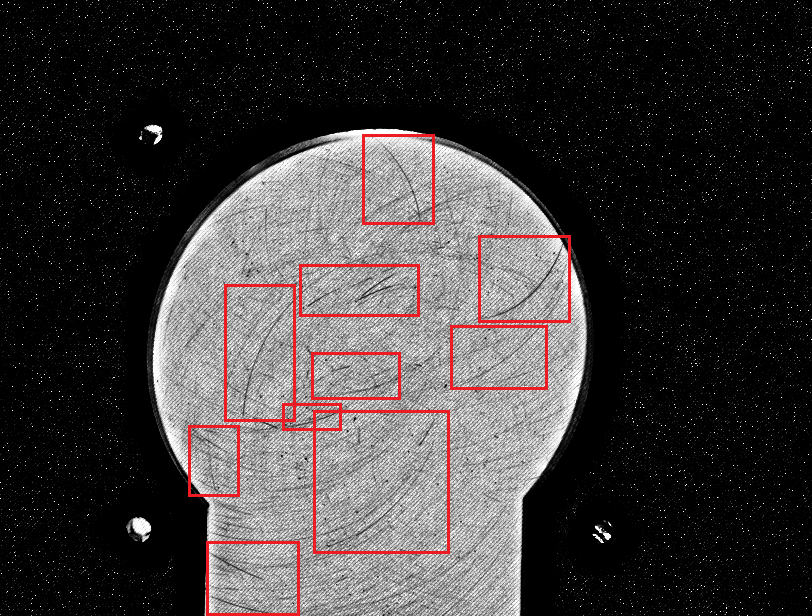
\includegraphics[width=.31\textwidth]{05_ergebnisse/ergSichtpruefungDurchLichtstreuung/durchlichtAuswertungLichtstreuung/figures/polierfehler_ergebnis_verbessert}};
		\node [anchor=north west] (img3) at (0.69\textwidth,0) {\includegraphics[width=.31\textwidth]{05_ergebnisse/ergSichtpruefungDurchLichtstreuung/durchlichtAuswertungLichtstreuung/figures/HS_Beschädigung_ergebnis_verbessert}};
		
		% Captions
		\node [below=0.2cm of img1] (cap1) {Brillenglas 1};
		\node [below=0.2cm of img2] (cap2) {Brillenglas 2};
		\node [below=0.2cm of img3] (cap3) {Brillenglas 3};			
	\end{tikzpicture}
\end{adjustbox}
\caption[Verbesserung der Ergebnisbilder]{Verbesserung der Ergebnisbilder. In Grün: Gravur der Brillenglaskennzeichnung. In Rot: Kratzer und ähnliche Beschädigungen der Oberfläche.\footnotemark}
		\label{tikz:abbNachbearbeitung}
	\end{figure}
	\footnotetext{Es wurde nur eine Auswahl von Fehlstellen markiert, um die Übersicht beizubehalten.}
}

\noindent
In den einzelnen Teilbildern aus Abbildung \ref{tikz:abbNachbearbeitung} kann man in den markierten Bereichen Fehlstellen bzw. Gravuren als dunkle Formen erkennen.
Dadurch werden für das Brillenglas 1 und das Brillenglas 3 aus Abbildung \ref{tikz:abbNachbearbeitung} die eingravierten Markenzeichen auf den Oberflächen sichtbar.
In Brillenglas 2 erkennt man viele Kratzspuren die auf eine fehlerhafte Polierung hindeuten.